\subsection{From 1D to 2D}
After inspecting the 2D fast Fourier algorithm(FFT) we realized the algorithm shows a promising potential for parallelization. The steps for performing 2D FFT is as follows: 
\begin{itemize}
\item Perform row-wise FFT on each row of the image (can be done completely in parallel.)
\item Transpose the Image: This stage can be ommited and be replaced by column-wise FFT but since the memory access pattern is not efficient we transpose the image beforehand.
\item Perform row-wise FFT on each row of the transposed image(which is now the columns of the previous matrix)
\item Transpose the matrix once again to maintain the original order.
\end{itemize}
It should be clear now that if we consider a \(n * n \) image, n parallel process can do the required calculations for row-wise and then the column-wise FFT. While we can achieve a level of parallelism with a multi-core CPU, the speedup would not be significant as the number of cores are limited and hence the need for an accelerator can be felt.
\subsection{Moving the calculations to GPU}
What makes GPUs the perfect candidate for this problem is the massive parallelism they can provide because of their core count. As an example the test machine we used was shipped with an RTX3070 mobile GPU and offered 5120 NVIDIA CUDA cores. A number that is very impressive for an ordinary laptop. With that in mind we moved all the computations to GPU by implementing several CUDA kernels that can be found in \textit{FFTGPU.cu} and then wrappers that can be located in the \textit{FourierTransform.cpp}.
In the first implementation we implemented each step in a separate kernel:
\begin{itemize}
\item bit-reversal
\item 1D FFT
\item Transpose
\end{itemize}

Then in the wrapper \textit{IterativeFFTGPU2D} we would take the data from CPU, move it to GPU and launch the kernels with above order and after performing the calculations were done we moved the data back to the host and used opencv to check the correctness of our result in \textit{cuda\_main.cpp}.

\subsection{Block by block FFT}
Since one of our objectives was to perform image compression, we realized that most of the algorithms for compression(including JPEG used in out project) use 8x8 block transformations and do not perform transformations on the whole input at once. So with that in mind another implementation was done but this time each kernel was responsible for calculating operations on 8x8 elements not each row. In order to balance the computations the bit reversal and transposition was also done in the same kernel because profiling suggested that if we do otherwise each kernel would be so lightweight and also the number of kernels launched would become significantly large which would the GPUs scheduling performance. The implementation can be found in the class named \textit{BlockFFTGPU2D}

\subsection{Performance analysis}
After the initial implementation on the GPU we realized that only outperforms CPU for large images and performed worse for smaller inputs. After analyzing the performance using NVIDIA Nsight Systems software we realized that most of the GPU time is being spent on data transfers between host and device. 

\subsection{Performance improvements}
The solution that NVIDIA provided was overlapping the computations and memory transfers since these two operations could be executed in parallel. The tool that was provided was "Streams". Each kernel and it's related memory copies would be placed in a separate stream and then they would be interleaved based on their resource usage, for instance if a kernel was awaiting for data to be copied another kernel that had its data ready could utilize this dead time and be executed while the data for the other kernel was being copied.
\\
\par Another improvement that was done was utilizing device shared memory.The memory hierarchy in CUDA suggests that slowest to fastest memory are as follows: Global memory, per block shared memory, thread registers. In the initial implementation we were only using global memory which was significantly degrading the performance. In the later implmentation we used shared memory to store the data required for each block and perform the computations while they were still present on the shared memory and then later move them back to GPU's global memory. This significantly boosted the throuput of our application. In the bellow graphs generated by NVIDIA Nsight Systems you can observe how the overall runtime and memory access patterns are improved:

\begin{figure}[ht]
    \centering
    \subfigure[Non streamed with no shared memory kernel Launch]{\label{fig:fft_floats}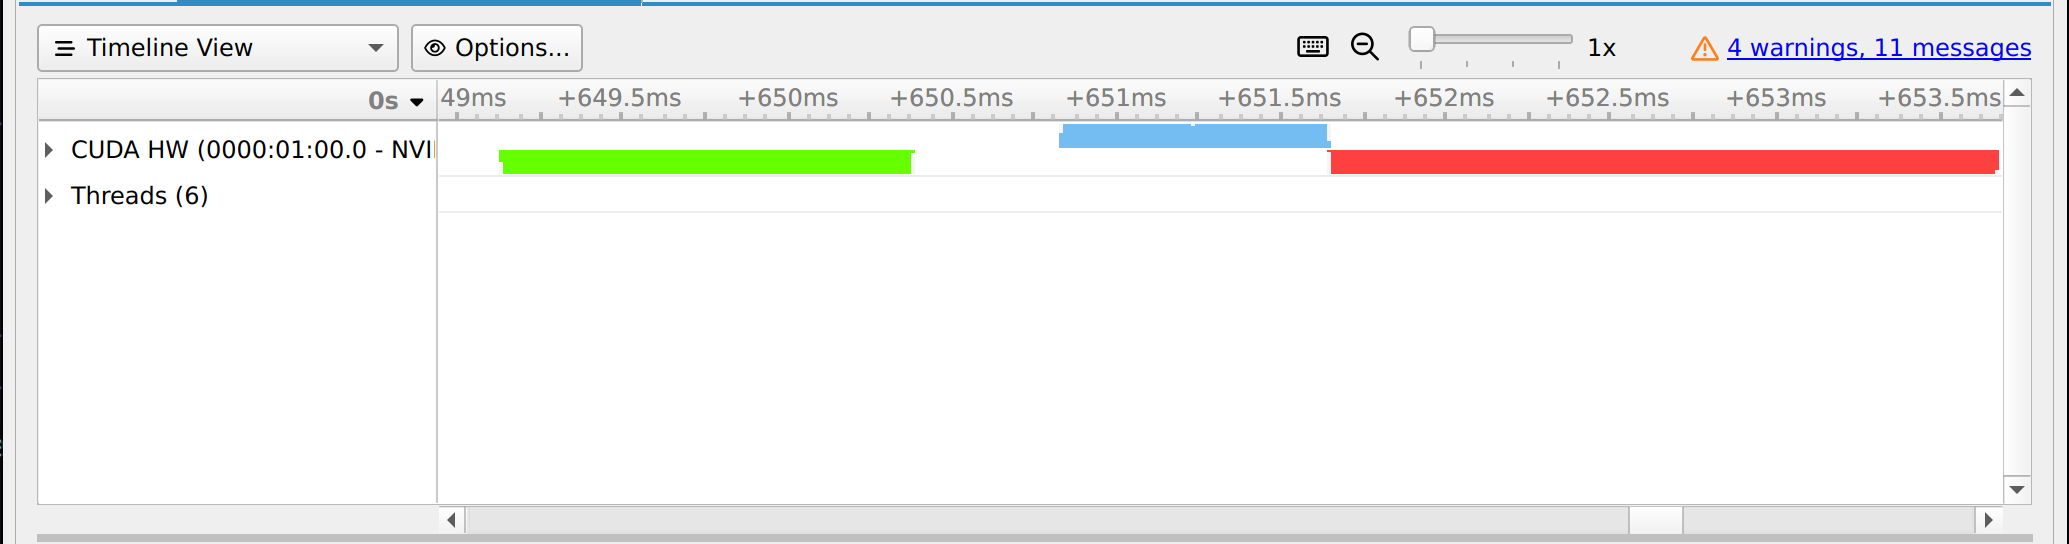
\includegraphics[width=120mm]{image/cuda_profile_non_stream.png}}
    \subfigure[Streamed kernel Launch with shared memory]{\label{fig:fft_doubles}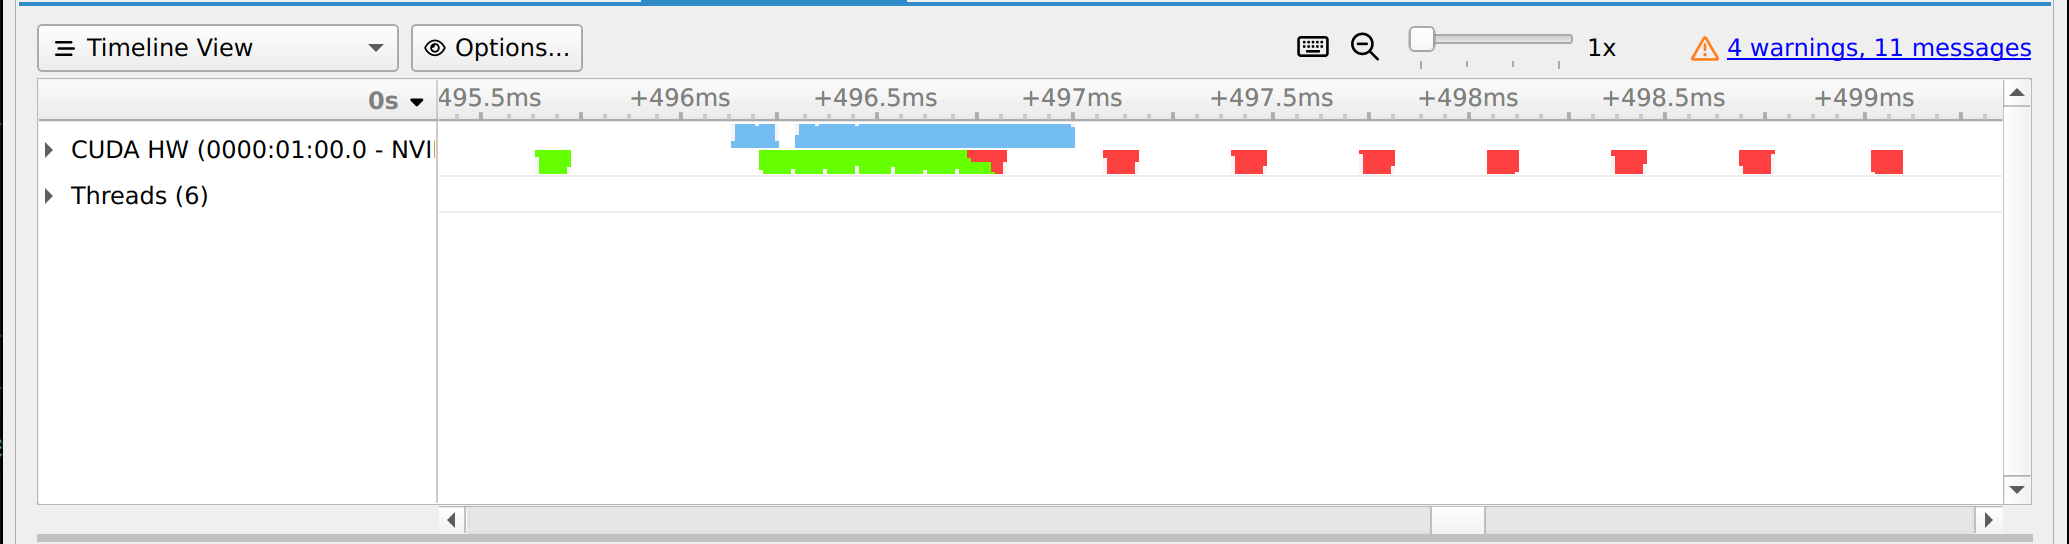
\includegraphics[width=120mm]{image/cuda_profile_stream.png}}
    \caption{The blue line indicates the time spent on processing, the green line indicates the time spent on host to device transfer and the red line shows device to host transfer times for the input image. The second test shows significant improvement in both overlapping the copies and processing and also overall reduced execution time}
    \label{fig:compression_road}
\end{figure}
